\chapter{AdaBoost}
\label{ch-adaboost}

This chapter
is based on Ref.\cite{wiki-adaboost}.


Adaptive Boosting (AdaBoost) is 
a method of constructing
a strong
classifier function
as a linear 
combination
of an ensemble
of weak classifier
functions.

Below,
we will abbreviate
``ensemble classifiers" by ``e-classifiers"
and ``weak classifiers' by ``w-classifiers".


Chapter \ref{ch-dtree}
defines decision trees (dtrees)
and explains how to construct them.
A
{\bf tree stump}
is a dtree  with only one
parent and 2 children nodes.
Usually the 
w-classifier functions
for AdaBoost
come from tree stumps
(because tree stumps
are w-classifiers
and simple to compute), but
the core
AdaBoost algorithm
is oblivious to 
where the w-classifier functions came from.


Chapter \ref{ch-rforest}
is on Bagging (Random Forest),
which is 
another method
besides AdaBoosting
of building a classifier function
from an ensemble 
of classifier functions.
These two methods are most commonly
applied to dtrees: AdaBoosting for an ensemble of
tree stumps, and Bagging for a random 
forest (which
is an ensemble
of dtrees that are usually much more
complicated than tree stumps). Both methods 
 are highly effective
in mitigating overfitting,
a common problem with simple
dtrees.


\section{AdaBoost for general ensemble
of w-classifiers}
In this 
section 
we discuss the core Adaboost
algorithm,
valid for a generic ensemble of w-classifiers.

Let $L=[0,1,2, \ldots, nsam-1]$ be a list of
individuals (samples) in a population.
In this chapter, we will use the notation 
$A^\s=A[\s]$ 
and $\vec{A}=[A^\s:\s\in L]$
for a  list (vector, 1-D  array) indexed by $L$.
We will refer to $DS=(\vec{x}, \vec{y})$ 
where $x^\s\in S_\rvx$, $y^\s\in S_\rvy$,
as a dataset. 
Let $T=\{0,1, \dots, nt-1\}$.
Let
$x=(x_0, x_1, \ldots, x_{nt-1})
\in S_{\rvx_0}\times S_{\rvx_1}
\times\ldots\times
 S_{\rvx_{nt-1}}=S_\rvx$.

AdaBoost assumes
that the classifier class set
$S_\rvy$  and
all the feature sets $S_{\rvx_t}$ 
are
binary:
$S_\rvy=S_{\rvx_t}=\{-1, 1\}$ for 
all $t\in T$.


Suppose that we are given an
ensemble of $nt$
{\bf w-classifiers}
$Y_t:S_\rvx\rarrow \{-1, 1\}$,
where $t\in T$.
Suppose we
 want to find  {\bf intermediate 
e-classifiers}
$\caly_t:S_\rvx\rarrow \RR$ 
given by 

\beq
\caly_t(x^\s)=
\sum_{t'\leq t}\alp_{t'}Y_{t'}(x^\s)
\eeq
for $t=0, 1, \ldots, nt-2$
and a {\bf final e-classifier}
given by 

\beq
\caly_{nt-1}(x^\s)=
\sum_{t=0}^{nt-1}\alp_t Y_t(x^\s)
\;.
\eeq
One can
turn  this final e-classifier
into a binary classifier 
like the $Y_t$
by using $sign(\caly_{nt-1})$.
The Adaboost algorithm 
yields a set of 
coefficients $\alp_t$
for which the final e-classifier
is much stronger (i.e., less error
prone) than any of the w-classifiers of the ensemble.

Note that
\beq
\caly_t(x^\s)=
\caly_{t-1}(x^\s)
+\alp_t Y_t(x^\s)
\eeq
for $t\in T$ if  we define
$\caly_{-1}=0$. Hence

\beq
\underbrace{e^{-y^\s \caly_t(x^\s)}}_
{Z_t w^\s_{t+1}}
=
\underbrace{e^{-y^\s \caly_{t-1}(x^\s)}}_
{Z_{t-1}w^\s_{t}}
e^{-\alp_t y^\s Y_t(x^\s)}
\eeq
where the {\bf weights}
$w_t^\s$ and 
and the {\bf
partition
function} $Z_t$ are defined by

\beq
w^\s_{t+1} = 
\left\{
\begin{array}{ll}
1/nsam&\text{for $t=-1$}
\\
\frac{\exp(-y^\s \caly_t(x^\s))}{Z_t}
&\text{for $t\geq 0$}
\end{array}
\right.
\eeq
and

\beq
Z_t =\sum_\s
e^{-y^\s \caly_t(x^\s)}
\;.
\eeq
Note that the probability
distribution 
$P(\s|t+1)=w^\s_{t+1}$
of weights 
at time $t+1$ emphasizes 
(i.e., gives higher probability to)
the errors (i.e., 
occurrences of $y^\s \caly_t(x^\s)=-1$
for some population
individual $\s$)
 of the previous (i.e., at time $t$)
intermediate 
e-classifier 
$\caly_t$.
In other words,
every new
intermediate 
e-classifier $\caly_{t+1}$
concentrates
on those individuals $\s$
on which the previous e-classifier $\caly_{t}$
performed poorly.

Note also 
the partition function $Z_t$
a good measure
of the {\bf classification error}
(i.e., 
occurrences of $y^\s \caly_t(x^\s)=-1$)
of $\caly_t$. We will
therefore use $Z_t$
for that purpose,
as an error measure.

For $t>1$, we have 
\beqa
Z_t
&=&
\sum_\s
e^{-y^\s \caly_t(x^\s)}
\\
&=&
\sum_\s 
\underbrace{e^{-y^\s \caly_{t-1}(x^\s)}}_
{Z_{t-1}w^\s_t}
e^{-\alp_t y^\s Y_t(x^\s)}
\\
&=&
Z_{t-1} E_\s[e^{-\alp_t y^\s Y_t(x^\s)}]
\eeqa
Define the {\bf success rate} by
\beqa
S_t&=&
\sum_\s w^\s_t\indi(y^\s Y_t(x^\s)=1)
\\
&=&
E_\s[\indi(\underbrace{y^\s Y_t(x^\s)=1}_
{\text{ iff }y^\s = Y_t(x^\s)}
)]
\eeqa
and the {\bf failure rate} by

\beqa
F_t&=&
\sum_\s w^\s_t\indi(y^\s Y_t(x^\s)=-1)
\\
&=& E_\s[\indi(
\underbrace{y^\s Y_t(x^\s)=-1}_
{\text{ iff }y^\s\neq Y_t(x^\s)}
)]
\;.
\eeqa
Note that 

\beq
S_t+F_t=1
\;,
\eeq
and

\beq
Z_t= Z_{t-1}(e^{-\alp_t}S_t
+
e^{+\alp_t}F_t)
\;.
\eeq

\begin{figure}[h!]
\centering
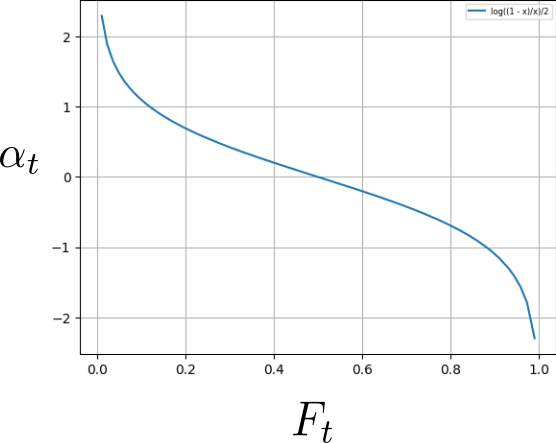
\includegraphics[width=3in]
{adaboost/adaboost-curve.png}
\caption{
Plot of function $\alp_t=
\frac{1}{2}\ln \frac{1-F_t}{F_t}$.
} 
\label{fig-adaboost-curve}
\end{figure}

We can find the $\alp_t$ values
that minimize the classification
error $Z_t$, and
then evaluate $Z_t$
at those optimum $\alp_t$ values:


\beq
\frac{d Z_t}{d\alp_t}
=Z_{t-1}(
-e^{-\alp_t}S_t
+
e^{\alp_t}F_t)
=0
\eeq

\beq
e^{2\alp_t}
=
\frac{S_t}{F_t}
\eeq

\beq
\alp_t=
\frac{1}{2}
\ln
\frac{S_t}{F_t}
=
\frac{1}{2}
\ln
\frac{1-F_t}{F_t}
\eeq

\beq
\frac{Z_t}{Z_{t-1}}=2\sqrt{S_tF_t}
=2\sqrt{(1-F_t)F_t}
\leq 1
\eeq
$f(x)=2\sqrt{(1-x)x}$
for $x\in[0,1]$
is dome shaped 
and its maximum 
is $1$,
which is
achieved iff $x=\frac{1}{2}$





\begin{figure}[h!]
$$
\xymatrix{
&
\rvY_0\ar[dr]\ar@/_1.5pc/[ddd]
&
\rvY_1\ar[dr]\ar@/_1.5pc/[ddd]
&
\rvY_2\ar[dr]\ar@/_1.5pc/[ddd]
&
\rvY_3\ar[dr]\ar@/_1.5pc/[ddd]
&
\rvY_4\ar@/_1pc/[ddd]
\\
(\vec{\rvx},\vec{\rvy})
\ar@/_1.5pc/[rr]
\ar@/_1.5pc/[rrr]
\ar@/_1.5pc/[rrrr]
\ar@/_1.5pc/[rrrrr]
&
\vec{\rvw}_0\ar[r]\ar[d]
&
\vec{\rvw}_1\ar[r]\ar[d]
&
\vec{\rvw}_2\ar[r]\ar[d]
&
\vec{\rvw}_3\ar[r]\ar[d]
&
\vec{\rvw}_4
\\
(\vec{\rvx},\vec{\rvy})
\ar@/_1.5pc/[r]
\ar@/_1.5pc/[rr]
\ar@/_1.5pc/[rrr]
\ar@/_1.5pc/[rrrr]
\ar@/_1.5pc/[rrrrr]
&
\ul{\alp}_0\ar[d]\ar[ru]
&
\ul{\alp}_1\ar[d]\ar[ru]
&
\ul{\alp}_2\ar[d]\ar[ru]
&
\ul{\alp}_3\ar[d]\ar[ru]
&
\ul{\alp}_4\ar[d]
\\
&
\ul{\caly}_0\ar[r]
&
\ul{\caly}_1\ar[r]
&
\ul{\caly}_2\ar[r]
&
\ul{\caly}_3\ar[r]
&
\ul{\caly}_4
}$$
\caption{Bnet for AdaBoost with
5 w-classifiers,
 $nt=5$.
All nodes labelled $(\vec{x},\vec{y})$
are the same node. 
}
\label{fig-aboost-bnet}
\end{figure}

The AdaBoost algo 
described
in this chapter is summarized
by
the bnet of Fig.\ref{fig-aboost-bnet}.
The TPMs, printed in blue, for the nodes of that
bnet, are as follows:

\beq\color{blue}
P(w^\s_0)=\frac{1}{nsam}
\;
\eeq
for all $\s$.

\beq\color{blue}
P(\vec{w}_{t+1}|\vec{w}_{t},
\alp_t, Y_t,    \vec{x}, \vec{y})=
\prod_\s
\indi(\;\;\; 
w^\s_{t+1} =\frac{ w^\s_t e^{-\alp_t y^\s Y_t(x^\s)}}
{\sum_\s numerator}
\;\;\;)
\eeq
for $t\geq 0$.


\beq\color{blue}
P(\alp_t|\vec{w}_t, \vec{x}, \vec{y})=
\indi(\;\;\; \alp_t=
\frac{1}{2}
\ln\frac{1-F_t}{F_t}
\text{ where }F_t=F_t(\vec{w}_t, \vec{x},\vec{y})\;\;\;) 
\eeq
for $t\in T$.

\beq\color{blue}
P(\caly_t| \caly_{t-1}, \alp_t, Y_t)
=
\indi(\;\;\;\caly_t= \caly_{t-1}+ \alp_t Y_t\;\;\;)
\eeq
for $t\in T$,
where $\caly_{-1}=0$.

\section{AdaBoost for ensemble of tree stumps}

Keep in mind that
AdaBoost assumes
$S_\rvy=S_{\rvx_t}=\{-1, 1\}$
for all $t\in T=\{0,1, \ldots, nt-1\}$.
In order to implement 
AdaBoost, we need to
specify 
$nt$
w-classifiers $Y_t:\{-1, 1\}^{nt}
\rarrow \{-1, 1\}$ for $t\in T$.
One can either
specify the $nt$ w-classifiers
a priori or build them
on-the-fly.

\begin{itemize}
\item {\bf
w-classifiers specified a priori}

Define a classifier 
for each feature $x_t$ 
where $t\in T$ by:

\beq
Y_t(x^\s)=x^\s_t\in \{-1, 1\}
\eeq
Hence, for this classifier,
$y^\s Y_t (x^\s)=y^\s x_t^\s$.

\item {\bf w-classifiers built
on-the-fly}

Recall
dataset
$(\vec{x},\vec{y})=
[(x^\s, y^\s):\s\in L]$
is indexed by the  list
 $L=[0, 1, \ldots, nsam-1]$.
If
$L_j$ is a list (possibly with 
duplicate items)
such that $set(L_j)\subset set(L)$,
 then
define
$DS_j=(\vec{x}, \vec{y})_{L_j}=
((x^\s)_{\s\in L_j}, 
(y^\s)_{\s\in L_j})$.
We will
refer to $DS_j$
as the {\bf restriction of 
$(\vec{x}, \vec{y})$ to $L_j$.}

The idea 
behind on-the-fly
w-classifiers is to choose 
$Y_t(x^\s)=x_t^\s$,
where $x_t$
is the feature with the largest
Gini in
the current dataset
$(\vec{x}, \vec{y})_{L_t}$.
To build 
$(\vec{x}, \vec{y})_{L_t}$,
we select at random 
from $L=[0, 1, \ldots, nsam-1]$,
a list $L_t$
of the same
length as $L$,
using the probability
distribution
$\vec{w}_{t-1}$.
By choosing
$L_t$
with
probabilities $\vec{w}_{t-1}$,
we emphasize 
individuals $\s$
that are failing.
Then
we define 
$(\vec{x},\vec{y})_{L_t}$
as the restriction of
$(\vec{x},\vec{y})$
to $L_t$.

Perhaps a causal diagram
will make all these 
new steps clearer
to the reader.
The bnet of 
Fig.\ref{fig-aboost-bnet-bags}
is a modification of the
 bnet
Fig.\ref{fig-aboost-bnet}
to include these new steps.
The TPMs,
printed in blue,
for new or changed nodes, are as 
follows:



\begin{figure}[h!]
$$
\xymatrix{
&
&L_1\ar[d]
&L_2\ar[d]
&L_3\ar[d]
&L_4\ar[d]
\\
&
(\vec{\rvx},\vec{\rvy})
\ar@/_1.5pc/[ddd]
\ar[d]
\ar[r]
\ar@/_1pc/[rr]
\ar@/_1pc/[rrr]
\ar@/_1pc/[rrrr]
&
(\vec{\rvx},\vec{\rvy})_{L_1}
\ar[d]
&
(\vec{\rvx},\vec{\rvy})_{L_2}
\ar[d]
&(\vec{\rvx},\vec{\rvy})_{L_3}
\ar[d]
&(\vec{\rvx},\vec{\rvy})_{L_4}
\ar[d]
\\
&
\rvY_0\ar[dr]\ar@/_1.5pc/[ddd]
&
\rvY_1\ar[dr]\ar@/_1.5pc/[ddd]
&
\rvY_2\ar[dr]\ar@/_1.5pc/[ddd]
&
\rvY_3\ar[dr]\ar@/_1.5pc/[ddd]
&
\rvY_4\ar@/_1pc/[ddd]
\\
(\vec{\rvx},\vec{\rvy})
\ar@/_1.5pc/[rr]
\ar@/_1.5pc/[rrr]
\ar@/_1.5pc/[rrrr]
\ar@/_1.5pc/[rrrrr]
&
\vec{\rvw}_0\ar[r]\ar[d]
\ar[uuur]
&
\vec{\rvw}_1\ar[r]\ar[d]
\ar[uuur]
&
\vec{\rvw}_2\ar[r]\ar[d]
\ar[uuur]
&
\vec{\rvw}_3\ar[r]\ar[d]
\ar[uuur]
&
\vec{\rvw}_4
\\
(\vec{\rvx},\vec{\rvy})
\ar@/_1.5pc/[r]
\ar@/_1.5pc/[rr]
\ar@/_1.5pc/[rrr]
\ar@/_1.5pc/[rrrr]
\ar@/_1.5pc/[rrrrr]
&
\ul{\alp}_0\ar[d]\ar[ru]
&
\ul{\alp}_1\ar[d]\ar[ru]
&
\ul{\alp}_2\ar[d]\ar[ru]
&
\ul{\alp}_3\ar[d]\ar[ru]
&
\ul{\alp}_4\ar[d]
\\
&
\ul{\caly}_0\ar[r]
&
\ul{\caly}_1\ar[r]
&
\ul{\caly}_2\ar[r]
&
\ul{\caly}_3\ar[r]
&
\ul{\caly}_4
}$$
\caption{Modification
of the bnet
of Fig.\ref{fig-aboost-bnet}
to include
on-the-fly
generation of
the w-classifiers.
}
\label{fig-aboost-bnet-bags}
\end{figure}

\beq\color{blue}
P(Y_t|(\vec{x}, \vec{y})_{L_t})=
\indi(\;\;\; Y_t(x^\s)=x^\s_t
\text{ where $x_t$ is
feature
in $(\vec{x},\vec{y})_{L_t}$ the
with lowest Gini.}
\;\;\;)
\eeq


\beq\color{blue}
P(L^\s_{t+1}=L^{\s'}|\vec{w}_t)=
w^{\s'}_t
\eeq

\beq\color{blue}
P((\vec{x}, \vec{y})_{L_t}|L_t,
(\vec{x},\vec{y}))
= 
\indi(\;\;\;
(\vec{x}, \vec{y})_{L_t}=
\text{  restriction of $(\vec{x},\vec{y})$ to $L_t$ }
\;\;\;)
\eeq
\end{itemize}


